\documentclass{beamer}
%
% Choose how your presentation looks.
%
% For more themes, color themes and font themes, see:
% http://deic.uab.es/~iblanes/beamer_gallery/index_by_theme.html
%
\mode<presentation>
{
  \usetheme{Madrid}      % or try Darmstadt, Madrid, Warsaw, ...
  \usecolortheme{seahorse} % or try albatross, beaver, crane, ...
  \usefonttheme{serif}  % or try serif, structurebold, ...
  \setbeamertemplate{navigation symbols}{}
  \setbeamertemplate{caption}[numbered]
} 


\usepackage[english]{babel}
\usepackage{kotex}
%\usepackage[utf8x]{inputenc}

\title[게임수학 - 수시고사6]{ 게임 수학 수시고사 6}
\author{강영민}
\institute{동명대학교}
\date{2015년 2학기}

\begin{document}

% Uncomment these lines for an automatically generated outline.
%\begin{frame}{Outline}
%  \tableofcontents
%\end{frame}


%%%%%%%%%%%%%%%%%%%%%%%%%%%%%%%%%%%%%%%%%%%%%%%%%%%%%%%%%


%%%%%%%%%%%%%%%%%%%%%%%%%%%%%%%%%%%%%%%%%%%%%%%%%%%%%%%%%
\begin{frame}{\small 수시고사 6 - 2015년 12월 1일 (화) $~~$ 학번:$~~~~~~~~~~~~~~~~~~$                이름:  }

\begin{tabular}{|p{11cm}|} \hline
다음과 같이 법선 $\mathbf N$을 가진 평면의 한 점에서 $\mathbf L$ 방향에서 빛이 떨어져서 $\mathbf R$ 방향으로 반사된다고 하자.
$\mathbf N$, $\mathbf L$을 안다면 이 $\mathbf R$을 어떻게 구할 수 있는지 설명하라.
\\ \hline \hline
\begin{figure}
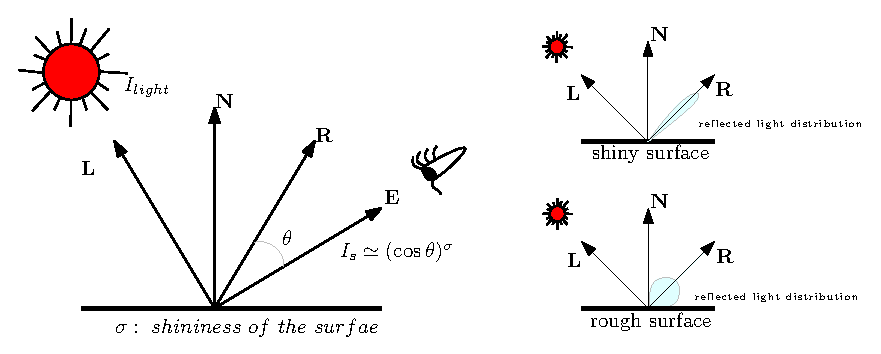
\includegraphics[width=5cm]{Math_lighting/specularConcept.eps}
\end{figure}
 \\ [20ex] \hline 
\end{tabular}

\end{frame}


%%%%%%%%%%%%%%%%%%%%%%%%%%%%%%%%%%%%%%%%%%%%%%%%%%%%%%%%%

\end{document}


